\textit{CUTE}, o ClUstering TrajectoriEs, è un algoritmo di clustering sovrapposto il cui obbiettivo è l'analisi
di gruppi di oggetti in movimento. 
Questa ricerca viene condotta considerando un insieme custom, nel numero e nella natura, di dimensioni.
Ad esempio è possibile considerare solamente la dimensioni collegate allo spazio-tempo
delle traiettorie oppure solo dimensioni semantiche (come ad esempio, le municipalità di una città), o ancora possono essere selezionati alcuni elementi da un gruppo e altri dall'altro.
CUTE può essere utilizzato per l'estrazione di pattern di co-movimento, considerando solamente la dimensione spaziale e quella temporale.

Lo scenario reale per la realizzazione di questo algoritmo è stata l'analisi condotta su
un insieme di traiettorie generate a Milano. 
All'interno di questo studio, i pattern di movimento sono stati analizzati a diversi livelli.
Una prima analisi è stata condotta dividendo la superficie della città in piccole celle:questa ricerca
ha rivelato i pattern di movimento del traffico, individuando quali potessero essere le strade
maggiormente frequentate.
Successivamente è stato realizzato uno studio basato sul vicinato: questo ha individuato i flussi di spostamento per specifiche categorie di utenti.
Infine una ricerca basata sulle municipalità ha mostrato quali fossero le aree della città più visitate da differenti gruppi di individui.

Questi casistiche hanno mostrato come al variare delle dimensioni considerate e della finezza della ricerca i risultati abbiano una natura totalmente diversa.
Lo scopo di CUTE è dunque di estrarre i pattern di movimento che avvengono con una certa soglia di frequenza.
CUTE si pone inoltre come obbiettivo l'integrazione di dimensioni custom e di scale personalizzabili così da riuscire a condurre più tipi di ricerche sfruttando lo stesso framework.

CUTE è etichettabile come algoritmo di \textit{colossal trajectory mining}.
L'idea alla base del colossal trajectory mining,
o mining di traiettorie su larga scala, interseca entrambi gli ambiti del clustering di traiettorie (\cref{subsec:trajectoryclustering})
e del colossal itemset mining.
Questa intersezione permette di sfruttare le potenzialità di entrambi gli approcci.
Scopo del mining di traiettorie colossali infatti è di individuare gruppi o cluster utilizzando i principi del colossal itemset mining.

In letteratura sono presenti esempi di tecniche a metà tra il mining di itemset frequenti e il clustering.
In particolare la ricerca di pattern di co-movimento presenta approcci ibridi di questo genere.
SPARE (\cref{sec:gcmp}) e \textit{GeT Move}~\cite{DBLP:journals/ijitdm/PhanPT16} implementano la ricerca di gruppi mischiando l'approccio basato su frequent itemset mining e il clustering.
Entrambi questi framework discretizzano il tempo in intervalli (\textit{bucket}) di dimensione finita.
Su questi poi applicano un clustering basato sulla densità o distanza.
Infine ricercano pattern di movimento mappando i vari oggetti come item e fondendoli in itemset sulla base del principio apriori.

Rispetto a quanto presentato fin d'ora, CUTE si pone come framework generico con le seguenti caratteristiche:

\begin{enumerate}
 \item \textbf{Ricerca di itemset su dataset ad alta dimensionalità}. Rispetto allo stato dell'arte, CUTE integra i principi e l'efficienza del
 mining di pattern colossali a traiettorie.
 Queste tecniche sono impiegate per individuare gruppi di oggetti definibili come pattern di co-movimento.
 
  \item \textbf{Sistema di riferimento generico}. A differenza degli altri algoritmi, 
  CUTE permette di utilizzare un insieme di dimensioni a scelta dell'utente per la ricerca di gruppi.
  Ad esempio è possibile impostare una ricerca esclusivamente basata sulle municipalità o la composizione del vicinato, senza includere 
  le dimensioni spazio-temporali.
  Oppure si può espandere la dimensione spazio temporale aggiungendo dati come l'altitudine oppure misure come velocità o accelerazione.
  Inoltre sono supportate dimensioni non esclusivamente monotone, come ad esempio i giorni della settimana.

  \item \textbf{Continuità rispetto al sistema di riferimento}. Nella ricerca di pattern di movimento è possibile specificare vincoli di contiguità su tutte le dimensioni impiegate.

  \item \textbf{Efficienza nel pruning}. La strategia di pruning impiegata permette di ridurre
  lo spazio di ricerca dell'algoritmo sulla base delle dimensioni utilizzate nel sistema di riferimento.

  \item \textbf{Implementazione distribuita}. CUTE mette a disposizione una soluzione distribuita per il problema del colossal trajectory mining compatibile con dataset costruiti su problemi del mondo reale.
\end{enumerate}



L'algoritmo segue tre passi per la formazione dei cluster, come anche rappresentato in~\cref{fig:chap-3:cute-overview}

  \begin{figure}
    \centering
    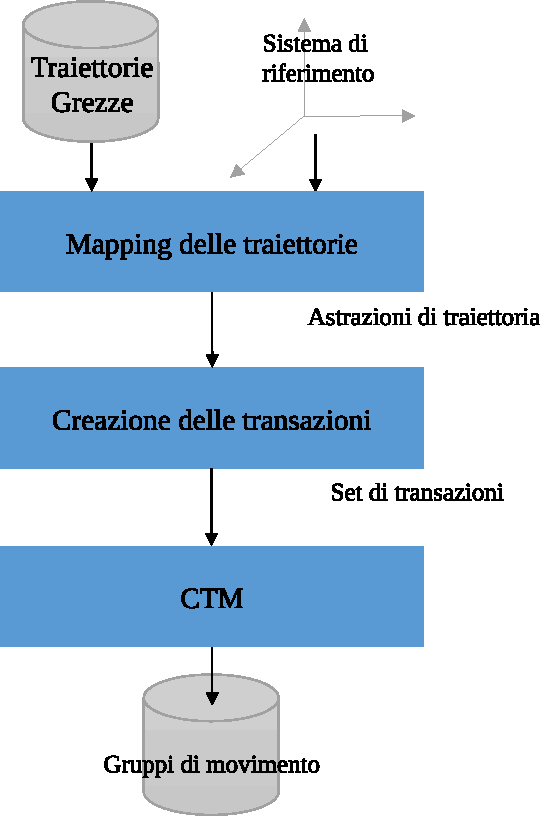
\includegraphics[width=.6\textwidth]{res/fig/sec-3/CUTEFlow.pdf}
    \caption{Rappresentazione grafica delle tre fasi dell'algoritmo CUTE}%
    \label{fig:chap-3:cute-overview}
  \end{figure}

  \begin{enumerate}
    \item \textbf{Mapping delle traiettorie}.

    In questo primo passo vengono analizzate le traiettorie presenti nel dataset. Da queste viene determinata la regione di movimento rispetto alle dimensioni impiegate.
    Successivamente quest'area viene divisa in un insieme di celle omogenee per dimensioni.
    A questo punto ad ogni traiettoria viene assegnato un insieme di celle secondo il seguente principio: una cella è attribuita ad una traiettoria quando quest'ultima ha
    almeno un punto che ricade entro i confini della cella.

    \item  \textbf{Creazione delle transazioni}.

    Durante questa fase vengono poste le basi per il mining di traiettorie: scopo di questa parte dell'algoritmo
    è infatti andare a generare l'insieme delle transazioni su cui verrà eseguita la ricerca di pattern.
    Ciò avviene considerando l'output della fase precedente e ribaltando la relazione traiettoria-cella.

    \item \textbf{Colossal Trajectory Mining}.

    Ultima e più importante passaggio dell'algoritmo, produce in uscita i pattern di movimento.
    Dato l'output della fase precedente, ovvero un insieme di transazioni appositamente creato,
    esegue una ricerca di itemset su dati ad alta dimensionalità.

  \end{enumerate}





